% Generated by code/needham.py -- do not edit by hand.
\definecolor{qocA}{rgb}{0.00,0.45,0.70}
\definecolor{qocB}{rgb}{0.90,0.60,0.00}
\definecolor{qocC}{rgb}{0.00,0.62,0.45}
\definecolor{qocD}{rgb}{0.80,0.40,0.00}
\definecolor{qocE}{rgb}{0.80,0.60,0.70}
\definecolor{qocF}{rgb}{0.35,0.70,0.90}
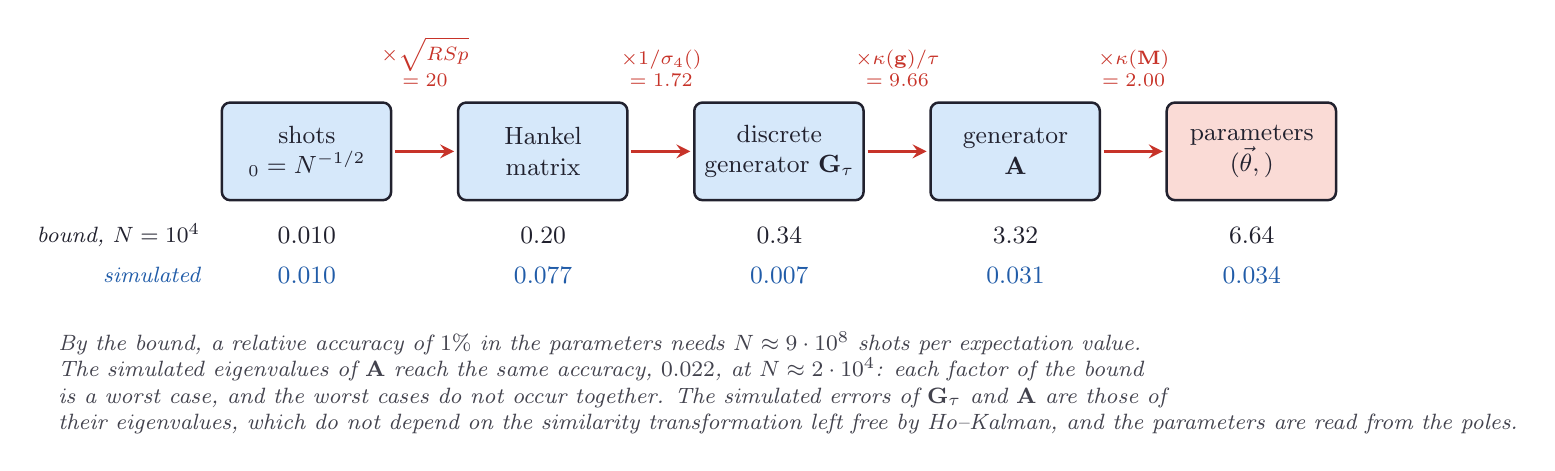
\begin{tikzpicture}[ink/.style={line width=0.9pt, ndInk}, faint/.style={line width=0.4pt, ndInk!35}, dashedink/.style={line width=0.5pt, ndInk!55, dash pattern=on 2.5pt off 2pt}, vec/.style={->, >=stealth, line width=1.2pt}, note/.style={font=\footnotesize\itshape, text=ndInk!85, align=center}, pointer/.style={->, >=stealth, line width=0.4pt, ndInk!60, shorten >=2pt, shorten <=1pt}, dot/.style={circle, fill=ndInk, inner sep=0pt, minimum size=3.4pt}, wash/.style={fill=ndSky, fill opacity=0.55}, every node/.style={text=ndInk}]
\definecolor{ndInk}{rgb}{0.13,0.13,0.18}
\definecolor{ndPaper}{rgb}{0.99,0.96,0.88}
\definecolor{ndSky}{rgb}{0.84,0.91,0.98}
\definecolor{ndRose}{rgb}{0.98,0.86,0.84}
\definecolor{ndBlue}{rgb}{0.13,0.36,0.66}
\definecolor{ndRed}{rgb}{0.78,0.20,0.16}
\definecolor{ndGold}{rgb}{0.88,0.62,0.10}
\definecolor{ndGreen}{rgb}{0.18,0.52,0.30}
\draw[ink, fill=ndSky, rounded corners=3pt] (2.30,-0.62) rectangle (4.45,0.62);
\node[font=\small, align=center] at (3.38,0) {shots\\ $\eps_0=N^{-1/2}$};
\draw[ink, fill=ndSky, rounded corners=3pt] (5.30,-0.62) rectangle (7.45,0.62);
\node[font=\small, align=center] at (6.38,0) {Hankel\\ matrix};
\draw[ink, fill=ndSky, rounded corners=3pt] (8.30,-0.62) rectangle (10.45,0.62);
\node[font=\small, align=center] at (9.38,0) {discrete\\ generator $\mathbf G_\tau$};
\draw[ink, fill=ndSky, rounded corners=3pt] (11.30,-0.62) rectangle (13.45,0.62);
\node[font=\small, align=center] at (12.38,0) {generator\\ $\mathbf A$};
\draw[ink, fill=ndRose, rounded corners=3pt] (14.30,-0.62) rectangle (16.45,0.62);
\node[font=\small, align=center] at (15.38,0) {parameters\\ $(\vec\theta,\Koss)$};
\draw[vec, ndRed] (4.50,0) -- (5.25,0);
\node[font=\scriptsize, text=ndRed, align=center, anchor=south] at (4.88,0.70) {$\times\sqrt{RSp}$\\ $=20$};
\draw[vec, ndRed] (7.50,0) -- (8.25,0);
\node[font=\scriptsize, text=ndRed, align=center, anchor=south] at (7.88,0.70) {$\times1/\sigma_4(\Hankel)$\\ $=1.72$};
\draw[vec, ndRed] (10.50,0) -- (11.25,0);
\node[font=\scriptsize, text=ndRed, align=center, anchor=south] at (10.88,0.70) {$\times\kappa(\mathbf g)/\tau$\\ $=9.66$};
\draw[vec, ndRed] (13.50,0) -- (14.25,0);
\node[font=\scriptsize, text=ndRed, align=center, anchor=south] at (13.88,0.70) {$\times\kappa(\mathbf M)$\\ $=2.00$};
\node[note, anchor=east, text=ndInk] at (2.15,-1.07) {bound, $N=10^4$};
\node[font=\small, text=ndInk] at (3.38,-1.07) {$0.010$};
\node[font=\small, text=ndInk] at (6.38,-1.07) {$0.20$};
\node[font=\small, text=ndInk] at (9.38,-1.07) {$0.34$};
\node[font=\small, text=ndInk] at (12.38,-1.07) {$3.32$};
\node[font=\small, text=ndInk] at (15.38,-1.07) {$6.64$};
\node[note, anchor=east, text=ndBlue] at (2.15,-1.57) {simulated};
\node[font=\small, text=ndBlue] at (3.38,-1.57) {$0.010$};
\node[font=\small, text=ndBlue] at (6.38,-1.57) {$0.077$};
\node[font=\small, text=ndBlue] at (9.38,-1.57) {$0.007$};
\node[font=\small, text=ndBlue] at (12.38,-1.57) {$0.031$};
\node[font=\small, text=ndBlue] at (15.38,-1.57) {$0.034$};
\node[note, anchor=north west, align=left] at (0.10,-2.17) {By the bound, a relative accuracy of $1\%$ in the parameters needs $N\approx9\cdot10^{8}$ shots per expectation value.\\ The simulated eigenvalues of $\mathbf A$ reach the same accuracy, $0.022$, at $N\approx2\cdot10^{4}$: each factor of the bound\\ is a worst case, and the worst cases do not occur together. The simulated errors of $\mathbf G_\tau$ and $\mathbf A$ are those of\\ their eigenvalues, which do not depend on the similarity transformation left free by Ho--Kalman,\ and the parameters are read from the poles.};
\end{tikzpicture}
